\newcommand{\entrynode}[0]{\ensuremath{\mathbf{entry}}}
\newcommand{\exitnode}[0]{\ensuremath{\mathbf{exit}}}
\section{Analysis of loop nesting forests}
\label{sec:part1:semantics:LNF}
As discussed above, the block sinking phase during $\lambda$-dropping
is governed by the (immediate) dominance relation between individual
basic blocks in the control flow graph. This section explores refined
placement strategies that arise from combining dominance structure
with additional CFG information, with a particular focus on the
nesting of loops. We sketch how the blocks of function declarations
for the immediate dominatees of a node can be refined and how the
resulting groups of functions can be placed in accordance with various
notions of \emph{loop nesting forests} from the literature. We first
treat reducible flow graphs before generalizing our analysis to
irreducible graphs.  Our treatment is not concerned with the
application of loop nesting forests to the calculation of dominance
relationships or phi-insertion points etc, but analyses how loop
nesting structure may be expressed declaratively in a functional
setting. As a consequence, our discussion assumes that both the
dominance tree and the CFG are available.

\subsection{Reducible control flow graphs}
\label{sec:part1:semantics:LNF:reducible}
Let us start with the simple dominance tree in
Figure~\ref{FigLoopAnalysis1ReducibleGraph}(a), showing a node $b$ and
its immediate dominance successors $b_1, \ldots, b_n$.  By the
definition of dominance, the control flow predecessors of each $b_i$
are amongst the nodes weakly dominated by $b$.
%: all control flow transfers to a $b_i$ originate in nodes dominated 
%by $b, b_1, \ldots, b_n$.

The standard placement strategy mentioned in the previous section
would represent this dominance structure
%(cf.~Section~\ref{section:Part1:Semantics:lambdaDropping:blockSinking})
using a single block of function declarations
\begin{equation}
\label{sec:SSA:functiondeclarationblock}
\begin{array}{l}
  \mathtt{function}\ f (\ldots)= 
  \mathtt{let} \ldots (* \mathit{body\ of\ f}*)\ldots \mathtt{in}\\
  \quad \begin{array}{rcl}
            \mathtt{function}\ f_1(\ldots) & = & e_1\\
             : \\
            \mathtt{and}\ f_n(\ldots) & = & e_n\\
            \mathtt{in}\ \ldots\ \mathtt{end}
        \end{array}
  \end{array}
\end{equation}
nested inside $f$. All $f_i$ would be treated identically, independent
of any control flow relationships between the basic blocks $b_1,
\ldots, b_n$. In particular, all function identifiers $f_i$ are
visible within all bodies $e_j$ and can also be called from within
$f$.

\begin{figure}
\begin{center}
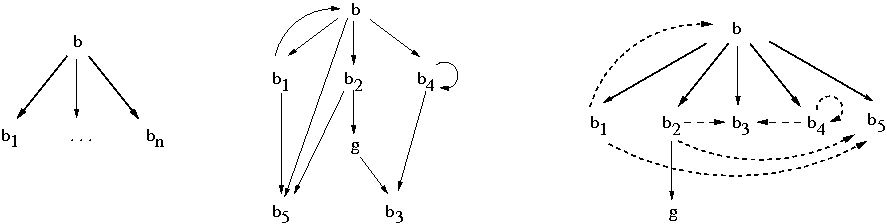
\includegraphics[scale=0.5]{loopAnalysis1}
\end{center}
\caption{\label{FigLoopAnalysis1ReducibleGraph} Placement for reducible flow graphs. (a) typical dominance tree (b) example control flow graph (c) overlay of CFG (dashed edges) onto dominance graph (solid edges) }
\end{figure}
A typical situation where this strategy is overly permissive is
indicated in the CFG in
Figure~\ref{FigLoopAnalysis1ReducibleGraph}(b). Here, node $b_3$ is a
join point of the paths $[b,b_2,g,b_3]$ and $[b,b_4,b_3]$ but cannot
be reached from any other $b_i$, and only indirectly from $b$.
Ideally, $b_3$ should not be visible from withing the declarations of
$b_1$, $b_5$ and the body of $b$. Node $b_5$ is a join point of the
paths $[b,b_1,b_5]$ and $[b,b_2,b_5]$ and is also an immediate
successor of $b$, but should not be visible from $b_3$, $b_4$, or $g$.

We refine the placement of functions underneath $b$ by overlaying CFG
information onto the dominance tree, as indicated in
Figure~\ref{FigLoopAnalysis1ReducibleGraph}(c). The graph captures the
call structure between the dominance trees underneath the immediate
dominatees of $b$, treating each $b_i$ as the representation of its
dominatees. For example, the source of the CFG edge $g \to b_3$ is
``moved up'' and captured by the dashed edge from $g$'s immediate
dominator, $b_2$, to $b_3$. In the following, we occasionally omit the
dominance levels below the $b_i$ when drawing overlay graphs, thus
emphasizing the fact that the links between the $b_i$ are intended to
capture the relationships between the dominance subtrees underneath
these nodes.
%Note that
%only sources of CFG edges need to be ``moved up'' in this fashion
%while their sinks are necessarily amongst the immediate dominatees of
%$b$ (including $b$), by the definition of the dominance relationship.

For reducible flow graphs, only trivial loops exist between the
dominance subtrees: the overlay graph is acyclic if we ignore
self-loops and loops involving the common dominator $b$.  We perform a
post-order-DFS (or more generally a reverse topological ordering)
amongst the $b_i$, ignoring self loops and back edges to $b$. In our
example, a possible order is $[b_5,b_1,b_3,b_2,b_4]$.  Staggering the
function declarations for these nodes according to this order yields
\begin{equation}
\label{FunctionalCascadeFun}
\begin{array}{l}
  \mathtt{function}\ f (\ldots)= 
  \mathtt{let} \ldots (* \mathit{body\ of\ f}*)\ldots \mathtt{in}\\
  \quad \begin{array}{l}
          \mathtt{function}\ f_5(\ldots) = e_5\\ \mathtt{in}\  
          \begin{array}[t]{l}
            \mathtt{function}\ f_1(\ldots) = e_1\ 
                 (* \mathit{contains\ calls\ to\ f\ and\ f_5}*) \\ \mathtt{in}\ 
            \begin{array}[t]{l}
              \mathtt{function}\ f_3(\ldots) = e_3\\ \mathtt{in}\ 
              \begin{array}[t]{l}
                \mathtt{function}\ f_2(\ldots) =
                 \begin{array}[t]{l}
                    \mathtt{let} \ldots (* \mathit{body\ of\ f_2}*)\ldots
                      \mathtt{in}\\
                     \quad \begin{array}{l}
                        \mathtt{function}\ g(\ldots) = e_g\
                           (* \mathit{contains\ call\ to\ f_3}*)\\ 
                        \mathtt{in}\   \ldots 
                              (* \mathit{calls\ to\ f_5\ and\ g} *)
                        \ldots \mathtt{end}
                     \end{array}\\
                   \end{array}\\ \mathtt{in}\
                \begin{array}[t]{l}
                  \mathtt{function}\ f_4(\ldots) = e_4\
                    (* \mathit{contains\ calls\ to\ f_3\ and\ f_4}*) \\
                   \mathtt{in} \ldots 
                      (* \mathit{calls\ to\ f_1, f_2, f_4, f_5}*)
                   \ldots \mathtt{end}
                \end{array}
              \end{array}
            \end{array}
          \end{array}
        \end{array}
  \end{array}
\end{equation}
The block of function declarations from
code~(\ref{sec:SSA:functiondeclarationblock}) has been replaced by a
cascade that still respects dominance structure (all $f_i$ are nested
inside $f$, and $g$ is nested inside $f_2$) but restricts the
visibility of function names: for example, $f_1$ is not visible within
$e_5$, and $f_3$ is not accessible from $f_1$ or $f_5$, as
desired\footnote{On the other hand, we note that $f_5$ remains visible
from within $f_3$ and $f_4$. Choosing a different topological order,
such as $[b_3,b_4,b_5,b_2,b_1]$, reverses the situation, i.e.~renders
$f_5$ inaccessible from $f_3$ or $f_4$, but leaves $f_3$ visible from
$f_1$ and $f_5$. Thus, the cascade of function declaration blocks is
not determined uniquely by the combined dominance and CFG structure.}.
As the reordering does not move function declarations \emph{inside}
each other (in particular: no function declaration is brought into or
moved out of the scope of the formal parameters of any other function)
the reordering does not affect the potential to perform parameter
dropping.
%As a potential downside, the representation depends on the
%particular topological
%ordering chosen.
\\

Code~(\ref{FunctionalCascadeFun}) may also be represented using
function declarations with $\lambda$-abstraction \footnote{In contrast
  to the CPS representations discussed in
  Section~\ref{section:Part1:Semantics:Continuations} no additional
  continuation parameters are used, so the representation is still
  \emph{direct style}.}. The advantages of this variant are twofold:
first, it enables us to syntactically distinguish between recursive
functions (i.e.~loops) and non-recursive ones, using the distinction
between $\mathtt{let}$ and $\mathtt{letrec}$ present in many
functional languages. In this form, the above code is represented as
follows, where $p$, $p_i$ represent the formal parameters of $f$,
$f_i$, respectively:
\begin{equation}
\label{FuntionalCascadeFun}
\begin{array}{l}
  \mathtt{letrec}\ f = \lambda\; p.\;
  \mathtt{let} \ldots (* \mathit{body\ of\ f}*)\ldots \mathtt{in}\\
  \quad \begin{array}{l}
          \mathtt{let}\ f_5 = \lambda\; p_5.\; e_5\\ \mathtt{in}\  
          \begin{array}[t]{l}
            \mathtt{let}\ f_1 = \lambda\;  p_1.\; e_1\ 
                 (* \mathit{contains\ calls\ to\ f\ and\ f_5}*) \\ \mathtt{in}\ 
            \begin{array}[t]{l}
              \mathtt{let}\ f_3 = \lambda\; p_3.\; e_3\\ \mathtt{in}\ 
              \begin{array}[t]{l}
                \mathtt{let}\ f_2 = \lambda\; p_2.\;
                 \begin{array}[t]{l}
                    \mathtt{let} \ldots (* \mathit{body\ of\ f_2}*)\ldots
                      \mathtt{in}\\
                     \quad \begin{array}{l}
                        \mathtt{let}\ g = \lambda\; p_g.\; e_g\
                           (* \mathit{contains\ call\ to\ f_3}*)\\ 
                        \mathtt{in}\   \ldots 
                              (* \mathit{calls\ to\ f_5\ and\ g} *)
                        \ldots \mathtt{end}
                     \end{array}\\
                   \end{array}\\ \mathtt{in}\
                \begin{array}[t]{l}
                  \mathtt{letrec}\ f_4 = \lambda\; p_4.\; e_4\
                    (* \mathit{contains\ calls\ to\ f_3\ and\ f_4}*) \\
                   \mathtt{in} \ldots 
                      (* \mathit{calls\ to\ f_1, f_2, f_4, f_5}*)
                   \ldots \mathtt{end}
                \end{array}
              \end{array}
            \end{array}
          \end{array}
        \end{array}
  \end{array}
\end{equation}
Only the toplevel function $f$ and function $f_4$ are recursive.

Second, the use of $\lambda$-abstractions enables us to further
restrict the visibility of function names. Indeed, while $b_3$ is
immediately dominated by $b$, its only control flow predecessors are
$b_2/g$ and $b_4$. We would hence like to make the declaration of
$f_3$ local to the \emph{tuple} $(f_2, f_4)$, i.e.~invisible to $f$.
This can be achieved by combining $\mathtt{let}$/$\mathtt{letrec}$
binding with pattern matching, as we may insert the shared declaration
of $f_3$ \emph{between} the declaration of the names $f_2$ and $f_4$
and the $\lambda$-bindings of their formal arguments:

\begin{equation}
\label{FuntionalCascadeFunLambda}
\begin{array}{l}
  \mathtt{letrec}\ f = \lambda\; p.\;
  \mathtt{let} \ldots (* \mathit{body\ of\ f}*)\ldots \mathtt{in}\\
  \quad \begin{array}{l}
          \mathtt{let}\ f_5 = \lambda\; p_5.\; e_5\\ \mathtt{in}\  
          \begin{array}[t]{l}
            \mathtt{let}\ f_1 = \lambda\;  p_1.\; e_1\ 
                 (* \mathit{contains\ calls\ to\ f\ and\ f_5}*) \\ \mathtt{in}\ 
            \begin{array}[t]{l}
                \mathtt{letrec}\ (f_2, f_4) =\\ 
                 \quad 
                 \begin{array}{l}
                   \mathtt{let}\ f_3 = \lambda\; p_3.\; e_3\\ \mathtt{in}\ 
                   \begin{array}[t]{l}
                   (\lambda\; p_2.\; 
                       \begin{array}[t]{l}
                         \mathtt{let} \ldots (* \mathit{body\ of\ f_2}*)\ldots
                         \mathtt{in}\\
                         \quad \begin{array}{l}
                           \mathtt{let}\ g = \lambda\; p_g.\; e_g\
                              (* \mathit{contains\ call\ to\ f_3}*)\\ 
                           \mathtt{in}\   \ldots 
                                 (* \mathit{calls\ to\ f_5\ and\ g} *)
                           \ldots \mathtt{end},
                         \end{array}
                       \end{array}\\
                    \; \lambda\; p_4.\; e_4\
                       (* \mathit{contains\ calls\ to\ f_3\ and\ f_4}*))
                  \end{array}
                \end{array}\\
                \mathtt{in} \ldots 
                    (* \mathit{calls\ to\ f_1, f_2, f_4, f_5}*)
                 \ldots \mathtt{end}
            \end{array}
          \end{array}
        \end{array}
  \end{array}
\end{equation}
The recursiveness of $f_4$ is inherited by the function pair
$(f_2,f_4)$ but $f_3$ remains non-recursive\footnote{In OCaml, the
definition of recursive function tuples requires an explicit name for
the tuple and needs to be written using \emph{explicit} pattern
matching (or appropriate projections
$\mathit{fst}/\mathit{snd}$). Instead of writing
$$\begin{array}{l}
     \mathtt{letrec}\ (f_2, f_4) =
     %\\ \ quad
     \begin{array}[t]{l}
              \mathtt{let}\ f_3 = \lambda\; p_3.\; e_3\\ \mathtt{in}\ 
              \begin{array}[t]{l}
                   (\lambda\; p_2.\; \ldots 
                       (*\mathit{calls\ to} f_2, f_3, f_4*),\\
                   \; \lambda\; p_4.\; \ldots 
                       (*\mathit{calls\ to} f_2, f_3, f_4*))
              \end{array}
           \end{array}\\
     \mathtt{in} \ldots (*\mathit{calls\ to} f_2, f_4*)
  \end{array}
$$
one needs to write
$$\begin{array}{l}
     \mathtt{letrec}\ h =
     %\\ \ quad
     \begin{array}[t]{l}
              \mathtt{let}\ f_3 = \lambda\; p_3.\; e_3\\
              \mathtt{in\ match}\ h\ \mathtt{with}\ (f_2,f_4) \Rightarrow 
              \begin{array}[t]{l}
                   (\lambda\; p_2.\; \ldots 
                       (*\mathit{calls\ to} f_2, f_3, f_4*),\\
                   \ \lambda\; p_4.\; \ldots 
                       (*\mathit{calls\ to} f_2, f_3, f_4*))
              \end{array}\\
              \mathtt{end}
           \end{array}\\
     \mathtt{in\ match}\ h\ \mathtt{with}\ (f_2,f_4) \Rightarrow
           \ldots (*\mathit{calls\ to} f_2, f_4*)\ \mathtt{end}
  \end{array}
$$
where $h$ is a fresh function name.  
%In addition, function applications occasionally need to be $\eta$-expanded. 
%In order to simplify the presentation, we elide these details in the 
%remainder of this chapter, but provide in an appendix the working OCaml 
%code of a worked-out example. 
It should also be observed that standard execution models of
functional languages would allocate additional heap space for function
tuples such as $h$. While clearly significant in the context of
practical compilation, such operational aspects are orthogonal to the
focus on conceptual correspondences in the present chapter.}.  In
general, the role of $f_3$ is played by any merge point $b_i$ that is
not directly called from the dominator node $b$.

Declarations of explicit function tuples with $\lambda$-abstracted
parameter bindings and flexible insertion points for private function
declarations will prove useful in the following section, where we
treat functional representations of loop nesting forests for
irreducible control flow graphs.

\subsection{Irreducible control flow graphs}
For irreducible control flow graphs, the overlay graph is no longer
acyclic, even when self-loops and loops involving the common dominator
$b$ are ignored. For example, adding to the CFG from
Figure~\ref{FigLoopAnalysis1ReducibleGraph} the edges $b_5 \to b_1$
and $b_3 \to b_2$ leads to the two loops $[b_2,g,b_3]$ and $[b_1,b_5]$
that may both be entered by multiple paths from $b$ -- see
Figure~\ref{FigLoopAnalysis2IrreducibleGraph}(a).

\begin{figure}
\begin{center}
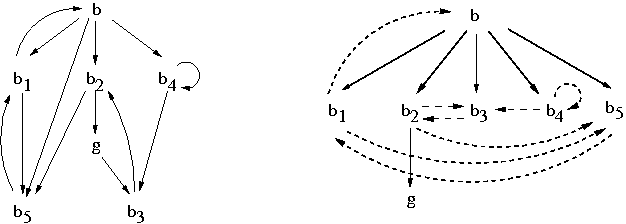
\includegraphics[scale=0.5]{loopAnalysis2}
\end{center}
\caption{\label{FigLoopAnalysis2IrreducibleGraph} control flow graph and overlay graph for irreducible graph}
\end{figure}
If we superimpose this CFG onto the (unchanged) dominance tree as
before we obtain the overlay graph in
Figure~\ref{FigLoopAnalysis2IrreducibleGraph}(b) which again contains
nontrivial cycles $[b_1,b_5]$ and $[b_2,b_3]$.

Generalizing the recipe from the previous section, one may perform the
reverse DFS/topological ordering on the partitioning of the overlay
graph into strongly connected components (SCC's). In the case of the
graph from Figure~\ref{FigLoopAnalysis2IrreducibleGraph} we obtain the
(in this case unique) ordering $[[b_1,b_5], [b_2,b_3], b_4]$, leading
to the staggered representation
\begin{equation}
\label{FunctionalCascadeIrredFun}
\begin{array}{l}
  \mathtt{function}\ f (\ldots)= 
  \mathtt{let} \ldots (* \mathit{body\ of\ f}*)\ldots \mathtt{in}\\
  \quad \begin{array}{l}
          \mathtt{function}\ f_5(\ldots) = e_5\ 
               (* \mathit{contains\ call\ to\ f_1} *) \\ 
          \mathtt{and}\ \ f_1(\ldots) = e_1\ 
                 (* \mathit{contains\ calls\ to\ f\ and\ f_5}*) \\ 
          \mathtt{in}\ 
            \begin{array}[t]{l}
              \mathtt{function}\ f_3(\ldots) = e_3\   
                 (* \mathit{contains\ call\ to\ f_2} *) \\
              \mathtt{and}\ f_2(\ldots) =
                 \begin{array}[t]{l}
                    \mathtt{let} \ldots (* \mathit{body\ of\ f_2}*)\ldots
                      \mathtt{in}\\
                     \quad \begin{array}{l}
                        \mathtt{function}\ g(\ldots) = e_g\
                           (* \mathit{contains\ call\ to\ f_3}*)\\ 
                        \mathtt{in}\   \ldots 
                              (* \mathit{calls\ to\ f_5\ and\ g} *)
                        \ldots \mathtt{end}
                     \end{array}\\
                   \end{array}\\ \mathtt{in}\
                \begin{array}[t]{l}
                  \mathtt{function}\ f_4(\ldots) = e_4\
                    (* \mathit{contains\ calls\ to\ f_3\ and\ f_4}*) \\
                   \mathtt{in} \ldots 
                      (* \mathit{calls\ to\ f_1, f_2, f_4, f_5}*)
                   \ldots \mathtt{end}
                \end{array}
          \end{array}
        \end{array}
  \end{array}
\end{equation}
(or similar code using $\lambda$-abstracted function declarations).

In general, the representation depends not only on the chosen
topological order as before, but also on the selection of SCC's.
Indeed, the above overlay graph only partitions uniquely into the two
non-trivial loops because the CFG loops do not overlap. For the
general case in which loops share nodes (or even edges), several
notions of loop have emerged in the imperative/SSA world, as outlined
in Chapter~\ref{}. A unifying perspective on these notions is provided
by Ramalingam's classification based on loop nesting
forests~\cite{DBLP:journals/toplas/Ramalingam02}.

In the following, we outline a functional interpretation of
Ramalingam's perspective by giving functional code for the various
loop partitioning schemes. In order to facilitate an easy comparison
with the original literature, our discussion employs the same running
example as Ramalingam's exposition, shown in
Figure~\ref{FigLoopAnalysisRamalingamCFG}. The CFG contains a node
$\entrynode$ that dominates five other nodes, $u$, $v$, $w$, $x$,
$\exitnode$ among which multiple overlapping loops exist. In addition
to the CFG, we again show the overlay graph that superimposes the CFG
onto the dominator tree.

\begin{figure}
  \begin{center}
    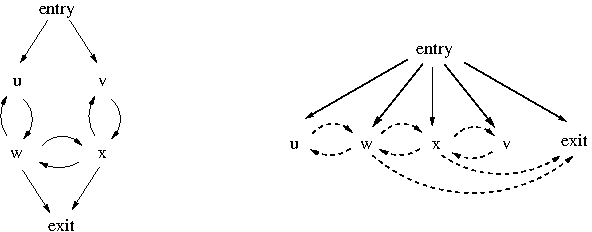
\includegraphics[scale=0.5]{Ramalingam}
  \end{center}
  \caption{\label{FigLoopAnalysisRamalingamCFG} Irreducible CFG with
    multiple overlapping loops (from
    Ramalingam~\cite{DBLP:journals/toplas/Ramalingam02}). 
    (a) CFG (b) overlay of CFG onto dominator tree}
\end{figure}

In Ramalingam's framework, a loop $L = (B,H)$ is comprised of two sets
of nodes $B$ and $H$ representing the \emph{body} -- all constituents
of the loop, i.e.~a (nontrivial) SCC -- and the \emph{headers},
respectively, with $\emptyset \neq H \subseteq B$ such that headers $h
\in H$ are not dominated by any vertex $b \in B \setminus \{h\}$. A
\emph{loop nesting forest} of a graph $G$ is a collection of loops
such that each nontrivial SCC of $G$ is covered by at least one loop
body and that the bodies $B_i$, $B_j$ of different loops ($i \neq j$)
are either disjoint or nested, i.e.~satisfy $B_i \cap B_j = \emptyset$
or $B_i \subseteq B_j$ or $B_j \subseteq B_i$.

A constructive characterization of loop nesting forests for $G$ may be
obtained by iterating the following process for $i=0,1,\ldots$, given
some header function $\mathcal{H}$ that associates headers to bodies
and may be instantiated to yield various preexisting notions of loop
nesting forests in the literature: at stage $i$, (a) identify the
(maximal) SCC's $B^i_1, \ldots B^i_{n_i}$ of the graph; (b) each
$B^i_j$ constitutes the body of a new outermost loop $L^i_j = (B^i_j,
H^i_j)$ with header set $H^i_j = \mathcal{H}(B^i_j)$; (c) remove from
$G_i$ the \emph{loopback edges} of loops $L^i_j$, i.e.~all edges from
$B^i_j$ to $H^i_j$; (d) repeat the process for the resulting graph
$G_{i+1}$. The thus obtained collection of loops $L^i_j$ constitutes a
loop nesting forest of $G = G_0$.

In the example program, the (single) maximal SCC is $B^0_1 = \{u, v,
w, x\}$.  The algorithm hence identifies a unique outermost loop $L_1$
comprised of these nodes.  Depending on the choice of header function
$\mathcal{H}$, different loop nesting forests arise.

\begin{description}

\item[Steensgaard] Steensgaard's construction instantiates the general
  scheme by choosing $\mathcal{H}(B)$ to yield the set of entry nodes
  of $B$, i.e.~the nodes in $B$ that have a predecessor outside $B$ in
  $G$. As is shown in
  Figure~\ref{FigLoopAnalysisRamalingamSteensgaard}(a), the first
  iteration of the algorithm thus identifies loop $L^0_1=(\{u,v,w,x\},
  \{u,v\})$.  Removing $L^0_1$'s loopback edges $w \to u$ and $x \to
  v$ from $G$ yields graph $G_1$, whose (only) SCC $\{w,x\}$ yields in
  the second iteration loop $L^1_1 = (\{w,x\}, \{w,x\})$.  Removing
  $L^1_1$'s loopback edges from $G_1$ results in the acyclic graph
  $G_2$, terminating the algorithm.  The resulting loop nesting forest
  for $G$ is shown in
  Figure~\ref{FigLoopAnalysisRamalingamSteensgaard}(b).  Loops
  (indicated as ellipses, decorated by with their header nodes) are
  nested according to the containment relation of bodies ($B^1_1
  \subseteq B^0_1$), with basic blocks being indicated using enclosing
  boxes.

  \begin{figure}
    \begin{center}
    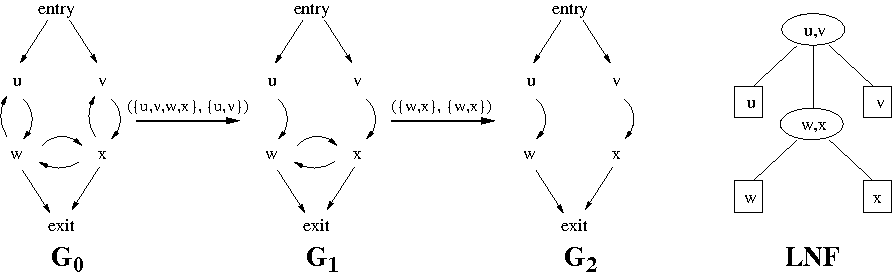
\includegraphics[scale=0.4]{RamalingamSteensgaard}
    \end{center}
    \caption{\label{FigLoopAnalysisRamalingamSteensgaard} Construction
       of Steensgaard's loop nesting forest for the CFG given in
       Figure~\ref{FigLoopAnalysisRamalingamCFG} (from
       Ramalingam~\cite{DBLP:journals/toplas/Ramalingam02}). 
       (a) Iterative construction of graphs $G_1$ and $G_2$; 
       (b) resulting loop nesting forest.}
  \end{figure} 

  In the functional representation, each identified loop $L=(B,H)$
  with headers $H=\{h_1,\ldots,h_n\}$ yields a function declaration
  tuple for functions $h_1,\ldots,h_n$, with private declarations for
  the non-headers from $B \setminus H$. For example, loop $L^0_1$
  provides entry points for the headers $u$ and $v$ but does not
  expose its non-headers $w$ and $x$.  Instead, the internal loop
  $L^1_1$ comprised of $w$ and $x$ is nested inside the definition of
  $L^0_1$, in accordance with the structure from
  Figure~\ref{FigLoopAnalysisRamalingamSteensgaard}(b).  In order to
  enable access to $L^1_1$ from both $u$ and $v$, we place $L^1_1$
  inside $L^0_1$ according to the scheme from
  code~(\ref{FuntionalCascadeFunLambda}), between the declaration of
  the names $u$ and $v$ and the definition of the corresponding bodies
  (written using $\lambda$-abstraction). Loop $L^1_1$ in turn exposes
  the entry points $w$ and $x$ to its ancestor loop $L^0_1$ but hides
  node $\exitnode$, which it effectively dominates.  

  \begin{equation}
    \label{FunctionalSteensgaard}
     \begin{array}{l}
       \mathtt{function}\ \entrynode (\ldots)=\\ 
       \qquad \mathtt{let} \ldots (* \mathit{body\ of\ \entrynode}*)\ldots\\
       \qquad \mathtt{in}\ 
         \begin{array}[t]{l}
           \mathtt{letrec}\ (u,v) =\\
           \qquad \begin{array}[t]{l}
                     \mathtt{letrec}\ (w,x) =\\
                     \qquad \mathtt{let}\ \exitnode = \lambda p_{\mathit{exit}}.\ \ldots\\
                     \qquad \mathtt{in}\ 
                       \begin{array}[t]{l}
                          (%(*function\ w*)\\
                           \ \lambda p_w.\ \ldots (*\mathit{calls\ to\ u,\
                                            x,\ and\ \exitnode}\ *),\\ 
                           % \ (*function\ x*)\\ 
                           \ \, \lambda p_x.\ \ldots (*\mathit{calls\ to\ w,\  
                                            v,\ and\ \exitnode}\ *)\ )
                       \end{array}\\
                     \mathtt{in}\ 
                     \begin{array}[t]{l}
                       (%(*function\ u *)\
                         \lambda p_u.\ \ldots (*\mathit{call\ to\ w}\ *),\\ 
                        % \ (*function\ v *)\
                        \ \, \lambda p_v.\ \ldots (*\mathit{calls\ to\ x}\ *)\ )
                      \end{array}\\
                    \end{array}\\
                    \mathtt{in}\ \ldots (*\mathit{calls\ to\ u\ and\ v}\ *) \ldots
         \end{array}
       \end{array}
  \end{equation} 

  In cases where the algorithm identifies several SCC's in an
  iteration, these can necessarily be topologically ordered and the
  resulting loops can be staggered accordingly, similar to
  code~(\ref{FunctionalCascadeIrredFun}).

  \item[Sreedhar-Gao-Lee] 
    The construction by Sreedhar, Gao, and Lee instantiates
    Ramalingam's general scheme by choosing $\mathcal{H}(B)$ to yield
    those nodes from $B$ that are not strictly dominated in $G$ by any
    $b\in B$. In\footnote{As an entry node of $B$ can never be
    strictly dominated by $b \in B$, any Steensgaard header is
    necessarily also a Sreedhar-Gao-Lee header.} our example, $H^0_1 =
    B^0_1 = \{u, v, w, x\}$ and we obtain the acyclic graph $G_1$ and
    the loop nesting forest shown in
    Figure~\ref{FigLoopAnalysisRamalingamSreedhar}.

    \begin{figure}
      \begin{center}
        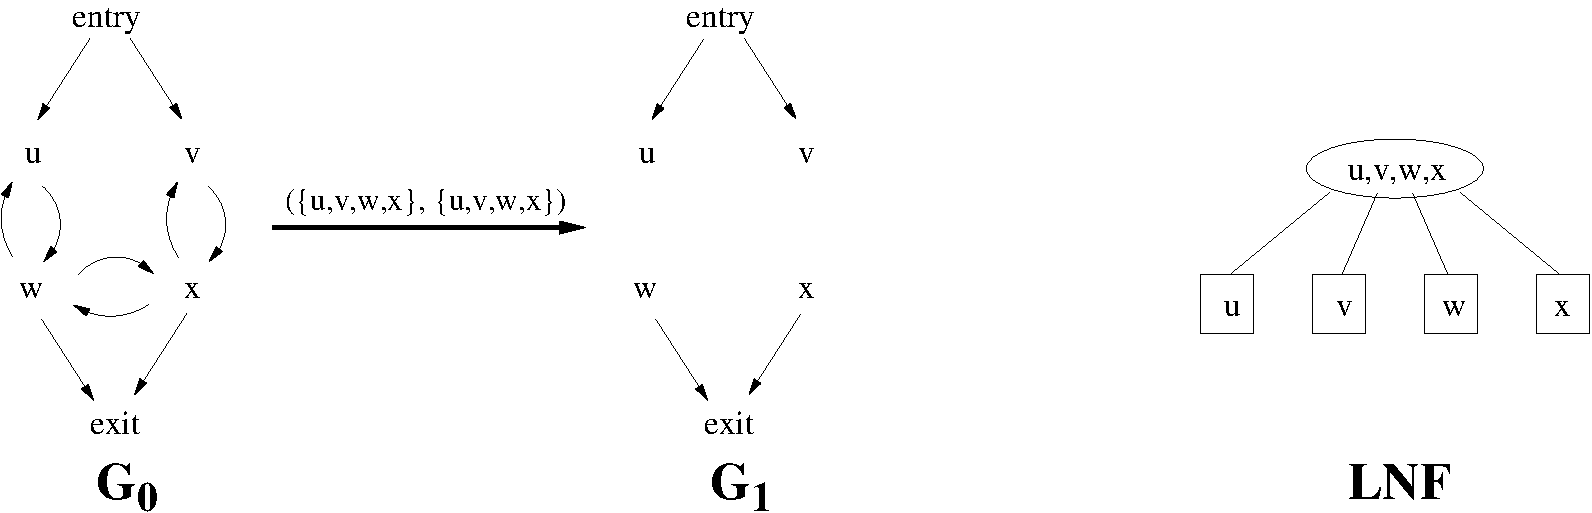
\includegraphics[scale=0.4]{RamalingamSreedhar}
      \end{center}
      \caption{\label{FigLoopAnalysisRamalingamSreedhar} Construction
        of the Sreedhar-Gao-Lee loop nesting forest for the CFG given
        in Figure~\ref{FigLoopAnalysisRamalingamCFG} (from
        Ramalingam~\cite{DBLP:journals/toplas/Ramalingam02}). (a) Iterative
        identification of graph $G_1$; 
        (b) resulting loop nesting forest.}
    \end{figure}

    Applying a similar interpretation of the forest as in
    Steensgaard's construction leads us to introduce a single 4-tuple
    of function declarations
    \begin{equation}
      \label{FunctionalSreedharGaoLee}
      \begin{array}{l}
        \mathtt{function}\ \entrynode (\ldots)=\\
        \qquad \mathtt{let} \ldots (* \mathit{body\ of\ \entrynode}*)\ldots\\ 
        \qquad \mathtt{in}\
        \begin{array}[t]{l}
          \mathtt{letrec}\ (u,v,w,x) =\\
          \qquad
          \begin{array}[t]{l}
            \mathtt{let}\ \exitnode = 
            \lambda p_{\mathit{exit}}.\ \ldots\\
            \mathtt{in}\ 
            \begin{array}[t]{l}
              (%(*function\ u *)\ 
              \lambda p_u.\ \ldots
              (*\mathit{call\ to\ w}\ *),\\
              % \ (*function\ v *)\
              \ \, \lambda p_v.\ \ldots
              (*\mathit{call\ to\ x}\ *),\\
              % \ (*function\ w*)\\ \
              \ \, \lambda p_w.\ \ldots
              (*\mathit{calls\ to\ u,\ x,\ and\ \exitnode}\ *),\\
              % \ (*function\ x*)\\
              \ \, \lambda p_x.\ \ldots
              (*\mathit{calls\ to\ w,\ v,\ and\ \exitnode}\ *)\ )
            \end{array}\\
          \end{array}\\
          \mathtt{in}\ \ldots (*\mathit{calls\ to\ u\ and\ v}\ *) \ldots
        \end{array}
      \end{array}
    \end{equation} 
    where we have again placed the declaration of $\exitnode$ inside
    that of the loop. Note that the representation exposes not only
    $u$ and $v$ to the surrounding code but also $w$ and $x$, despite
    the fact that the only calls to these functions occur inside the
    loop.  In this respect, the construction by Sreedhar, Gao, and Lee
    offers little advantage over a naive interpretation of the overlay
    graph from Figure~\ref{FigLoopAnalysisRamalingamCFG}(b) that does
    not differentiate between any members of the SCC $\{u,v,w,x\}$.

    \begin{figure}
      \begin{center}
        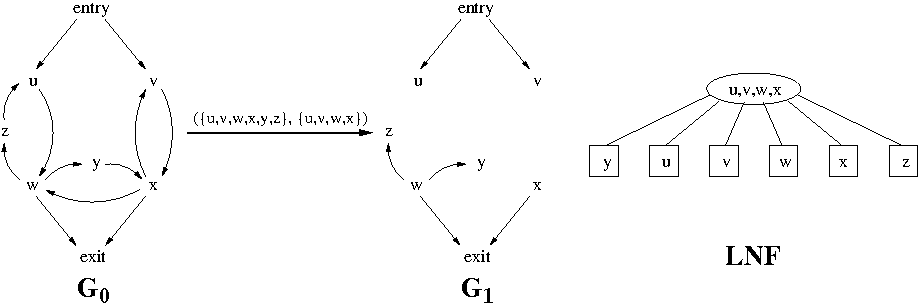
\includegraphics[scale=0.4]{RamalingamSreedharModified}
      \end{center}
      \caption{\label{FigLoopAnalysisRamalingamSreedharModified}
        Construction of a Sreedhar-Gao-Lee loop nesting forest for a
        variant of the CFG from
        Figure~\ref{FigLoopAnalysisRamalingamCFG}. (a) Iterative
        identification of graph $G_1$; (b) resulting loop nesting
        forest.}
    \end{figure}

    Continuing this comparison,
    Figure~\ref{FigLoopAnalysisRamalingamSreedharModified} shows a
    variation of our example program in which not all members of
    $L^0_1$ are Sreedhar-Gao-Lee headers. The additional nodes, $y$
    and $z$, are both dominated by $w$ and hence do not decorate the
    ellipsis in the loop nesting forest. A functional reading of this
    forest may either stagger the declarations of $y$ and $z$ next to
    that of $\exitnode$

    \begin{equation}
      \label{FunctionalSreedharGaoLee2}
      \begin{array}{l}
        \mathtt{function}\ \entrynode (\ldots)=\\
        \qquad \mathtt{let} \ldots (* \mathit{body\ of\ \entrynode}*)\ldots\\ 
        \qquad \mathtt{in}\
        \begin{array}[t]{l}
          \mathtt{letrec}\ (u,v,w,x) =\\
          \qquad
          \begin{array}[t]{l}
            \mathtt{let}\ \exitnode = \lambda p_{\mathit{exit}}.\ \ldots\
            \mathtt{in}\\
            \mathtt{let}\ z = \lambda p_z.\ \ldots\ (*\mathit{call\ to\ u}\ *)\
            \mathtt{in}\\
            \mathtt{let}\ y = \lambda p_y.\ \ldots\ (*\mathit{call\ to\ x}\ *)\\
            \mathtt{in}\ 
            \begin{array}[t]{l}
              (%(*function\ u *)\ 
              \lambda p_u.\ \ldots
              (*\mathit{call\ to\ w}\ *),\\
              % \ (*function\ v *)\
              \ \, \lambda p_v.\ \ldots
              (*\mathit{calls\ to\ x}\ *),\\
              % \ (*function\ w*)\\ \
              \ \, \lambda p_w.\ \ldots
              (*\mathit{calls\ to\ u,\ x,\ y,\ z,\ and\ \exitnode}\ *),\\
              % \ (*function\ x*)\\
              \ \, \lambda p_x.\ \ldots
              (*\mathit{calls\ to\ w,\ v,\ and\ \exitnode}\ *)\ )
            \end{array}\\
          \end{array}\\
          \mathtt{in}\ \ldots (*\mathit{calls\ to\ u\ and\ v}\ *) \ldots
        \end{array}
      \end{array}
    \end{equation} 
    or may place them inside the definition of $w$, exploiting the
    dominance relationship:
    \begin{equation}
      \label{FunctionalSreedharGaoLee3}
      \begin{array}{l}
        \mathtt{function}\ \entrynode (\ldots)=\\
        \qquad \mathtt{let} \ldots (* \mathit{body\ of\ \entrynode}*)\ldots\\ 
        \qquad \mathtt{in}\
        \begin{array}[t]{l}
          \mathtt{letrec}\ (u,v,w,x) =\\
          \qquad \begin{array}[t]{l}
            \mathtt{let}\ \exitnode = 
            \lambda p_{\mathit{exit}}.\ \ldots\\
            \mathtt{in}\
            \begin{array}[t]{l}
              (%(*function\ u *)\ 
              \lambda p_u.\ \ldots
              (*\mathit{call\ to\ w}\ *),\\
              % \ (*function\ v *)\
              \ \, \lambda p_v.\ \ldots
              (*\mathit{call\ to\ x}\ *),\\
              % \ (*function\ w*)\\ \
              \ \, \lambda p_w.\ 
              \begin{array}[t]{l}
                \mathtt{let}\ z = \lambda p_z.\ 
                \ldots\ (*\mathit{call\ to\ u}\ *)\ \mathtt{in}\\
                \mathtt{let}\ y = \lambda p_y.\
                \ldots\ (*\mathit{call\ to\ x}\ *)\\ \mathtt{in}\ 
                \ldots
                (*\mathit{calls\ to\ u,\ x,\ y,\ z,\ and\ \exitnode}\ *),
              \end{array}\\
              % \ (*function\ x*)\\
              \ \, \lambda p_x.\ \ldots
              (*\mathit{calls\ to\ w,\ v,\ and\ \exitnode}\ *)\ )
            \end{array}\\
          \end{array}\\
          \mathtt{in}\ \ldots (*\mathit{calls\ to\ u\ and\ v}\ *) \ldots
        \end{array}
      \end{array}
    \end{equation} 

    Again, the latter choice coincides with the placement suggested by
    the overlay graph, in which $y$ and $z$ are -- unlike $\exitnode$
    -- located in the subtree underneath $w$. In both cases, the
    relative order of $y$ and $z$ can be chosen arbitrarily.

  \item[Havlak] Finally, we consider Havlak's scheme for constructing
    loop nesting forests. The scheme is parametric in a DFS traversal
    of the CFG $G$ and instantiates Ramalingam's general scheme by
    choosing $\mathcal{H}(B)$ to yield the minimal node $b\in B$
    according to this order.

    Applying Havlak's construction to the running example using the
    DFS order $[\entrynode,u,w,\exitnode,x,v]$ yields a forest with
    three nested loops, each with a singleton header -- see
    Figure~\ref{FigLoopAnalysisRamalingamHavlak}.
    \begin{figure}
      \begin{center}
        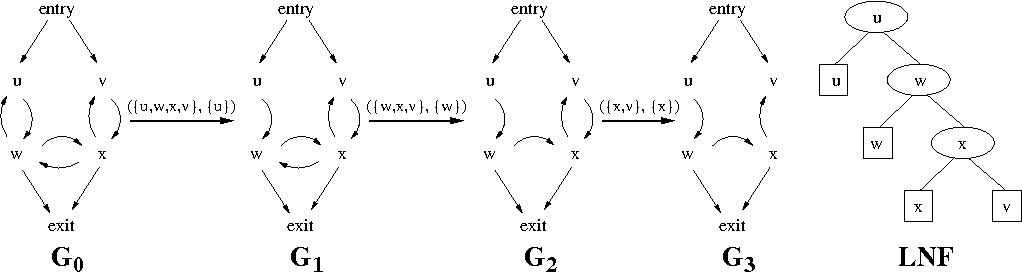
\includegraphics[scale=0.4]{RamalingamHavlak}
      \end{center}
      \caption{\label{FigLoopAnalysisRamalingamHavlak} Construction of
        a Havlak loop nesting forest for the CFG given in
        Figure~\ref{FigLoopAnalysisRamalingamCFG} (from
        Ramalingam~\cite{DBLP:journals/toplas/Ramalingam02}). (a) Iterative
        identification of graphs $G_1, G_2, G_3$; (b) resulting loop
        nesting forest.}
    \end{figure}

    In contrast to the constructions by Steensgaard and
    Sreedhar-Gao-Lee, Havlak-style header sets do not contain all
    entry nodes of a loop, hampering an elegant functional
    representation. As a case in point, our above functional reading
    of loop-nesting-forests cannot be directly applied to the LNF in
    Figure~\ref{FigLoopAnalysisRamalingamHavlak}(b) as the declaration
    of $v$ is buried inside $L^2_1$, making it inaccessible to its
    external caller $\entrynode$.

    While the nesting of loops in
    Figure~(\ref{FigLoopAnalysisRamalingamHavlak}) \emph{can} be
    reflected in a functional representation, the resulting code
    requires us to explicitly export the declaration of $v$ to the top
    level via additional tupled function declarations for the loops
    with headers $u$ and $w$, using the additional names\footnote{In
    OCaml, these exports have to be written in $\eta$-expanded form:
    for example, the export of $v'$ as $v''$ needs to be written as
    $\lambda p_{v''}.\ v'\ p_{v''}$.}  $v'$ and $v''$:

    \begin{equation}
    % file Havlak2, unfolding pairs of function declarations and 
    % including declaration of exit in natural place.
    \begin{array}{l}
      \mathtt{letrec}\ (u,v'') = \\ \qquad 
        \begin{array}{l}
          \mathtt{letrec}\ (w,v') =\\ \qquad
            \begin{array}{l}
              \mathtt{let}\ \exitnode =
                     \lambda p_{\mathit{exit}}.\ \ldots\ \mathtt{in}\\
              \mathtt{letrec}\ (x,v) = 
                (\begin{array}[t]{l}
                   \lambda p_x.\ \ldots (*\mathit{calls\ to\ w,\ 
                                          v,\ and\ \exitnode}\ *),\\
                   \lambda p_v.\ \ldots (*\mathit{call\ to\ x}\ *)\ )
                 \end{array}\\
              \mathtt{in}\
                (\begin{array}[t]{l}
                   \lambda p_w.\ \ldots (*\mathit{calls\ to\ u,\ 
                                          x,\ and\ \exitnode}\ *),\\
                   v\ (*\mathit{exporting}\ v\ \mathit{as}\ 
                         v'\ \mathit{here}*)\ )
                 \end{array}
            \end{array}\\
          \mathtt{in}\
             ( \begin{array}[t]{l}
                 \lambda p_u.\ \ldots (*\mathit{call\ to\ w}\ *),\\
                  v'\ (*\mathit{exporting}\ v'\ \mathit{as}\ 
                        v''\ \mathit{here}*)\ )
               \end{array}
        \end{array}\\
      \mathtt{in}\ \ldots (*\mathit{calls\ to\ u\ and\ v''}\ *) \ldots
    \end{array}
  \end{equation} 

  It thus appears that loop nesting forests according to Havlak
  (including the variant \emph{reduced Havlak forest} introduced by
  Ramalingam~\cite{DBLP:journals/toplas/Ramalingam02}) are less well
  suited for representation in a functional language than forests
  according to Steensgaard and Sreedhar-Gao-Lee.  
\end{description}
%\footnote{CHECK lazy patterns}
